\section{Preliminaries}

The \emph{stable matching} problem can be informally described as the task of pairing two sets of parties in such a way that 
no two unmatched parties should prefer each other over their assigned partners.
Stable matching problems have been typically framed in contexts such as matching men with women, students with universities, or producers with consumers.

\paragraph{Standard stable matching.}
% \paragraph{Traditional Stable Marriage.}
We consider a set of $n = 2k$ parties $\parties$, which are divided into two disjoint sets $L$ and $R$ with $|L| = |R| = k$: $L$ can represent, for instance, the set of men/students/producers while $R$ can represent the set of women/universities/consumers. 
In the \emph{stable matching problem}, every party $u$ in $L$ (resp.~$R$) has as input a \emph{preference list} (a permutation) $\preferences_u$ over the parties in $R$ (resp.~$L$).  We say that $u$ \emph{prefers} $v$ over $w$ if $v$ appears before $w$ in $\preferences_u$. In addition, $u$ prefers any party in its preference list $\preferences_{u}$ over being alone.

The objective of this problem
is to determine a \emph{stable matching}: a matching $M$ between $L$ and $R$ such that there is no \emph{blocking} pair.
A (non-matched) pair of parties $(u, v) \in L \times R$ is \emph{blocking} if $u$ and $v$ prefer each other compared to who they are currently matched to. 
Recall that parties always prefer being matched to being alone, so a pair of two unmatched parties on opposite sides is considered blocking.
This implicitly requires the matching to be \emph{maximal} (all parties are matched). 
It has been proven that 
a stable matching always exists, and it can be found using the Gale-Shapley algorithm $\GaleShapley$ \cite{GaleShapley}.
\begin{theorem}[\hspace{-1pt}{\cite{GaleShapley}}] \label{theorem:gale-shapley}
    There is a deterministic algorithm $\GaleShapley$ that takes as input the preference lists $\pi$ of all parties in $L$ and $R$ and returns a stable matching $M$.
\end{theorem}

\paragraph{Stable matching in a network.}
%\paragraph{The Tinder era (A distributed variant).} 
We now define the stable matching problem in a distributed setting. Here, the parties in $L \cup R$ are processors running a protocol over a network, exchanging messages via \emph{bidirectional authenticated communication channels}.
We assume that the network is \emph{synchronous}: the parties have synchronized clocks, and every message is delivered within a publicly known amount of time $\Delta$. This 
% usually
allows protocols to operate in rounds. As depicted in \cref{fig:communication-networks}, we will explore different network topologies, described below.


\begin{figure}[h]
    \centering
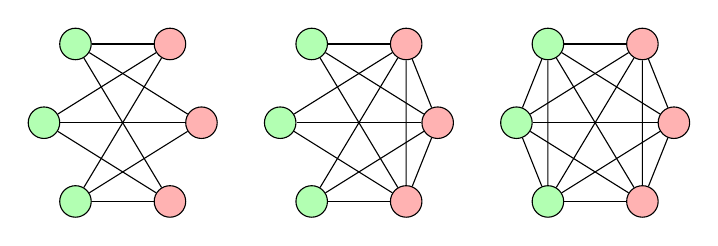
\begin{tikzpicture}[node distance=1.5cm, every node/.style={circle, draw,fill=red!30, minimum size=4mm}]
    % Bipartite communications
    \begin{scope}[local bounding box=graph1]
        % Left nodes
        \foreach \y in {0,2} {
            \node[fill=green!30] (L\y1) at (0.4,\y) {};
        }
        \node[fill=green!30] (L11) at (0,1) {};
        % Right nodes
        \foreach \y in {0,2} {
            \node (R\y1) at (1.6,\y) {};
        }
        \node (R11) at (2,1) {};
        % Edges between all left and right nodes
        \foreach \a in {0,1,2} {
            \foreach \b in {0,1,2} {
                \draw (L\a1) -- (R\b1);
            }
        }
    \end{scope}

    % One-sided communications
    \begin{scope}[shift={(3,0)}, local bounding box=graph2]
        % Left nodes
        \foreach \y in {0,2} {
            \node[fill=green!30] (L\y2) at (0.4,\y) {};
        }
        \node[fill=green!30] (L12) at (0,1) {};
        % Right nodes
        \foreach \y in {0,2} {
            \node (R\y2) at (1.6,\y) {};
        }
        \node (R12) at (2,1) {};
        % K_{3,3} edges
        \foreach \a in {0,1,2} {
            \foreach \b in {0,1,2} {
                \draw (L\a2) -- (R\b2);
            }
        }
        % Complete right subgraph
        \draw (R02) -- (R12) -- (R22) -- (R02);
    \end{scope}

    % Complete communications
    \begin{scope}[shift={(6,0)}, local bounding box=graph3]
        % Left nodes
        \foreach \y in {0,2} {
            \node[fill=green!30] (L\y3) at (0.4,\y) {};
        }
        \node[fill=green!30] (L13) at (0,1) {};
        % Right nodes
        \foreach \y in {0,2} {
            \node (R\y3) at (1.6,\y) {};
        }
        \node (R13) at (2,1) {};
        % K_{3,3} edges
        \foreach \a in {0,1,2} {
            \foreach \b in {0,1,2} {
                \draw (L\a3) -- (R\b3);
            }
        }
        % Complete left and right subgraphs
        \draw (L03) -- (L13) -- (L23) -- (L03);
        \draw (R03) -- (R13) -- (R23) -- (R03);
    \end{scope}
\end{tikzpicture}
\setlength{\belowcaptionskip}{-10pt}
\caption{The different kinds of communication networks we consider. From left to right: bipartite, one-sided and fully-connected networks. Note that even when communication is possible within $L$ or $R$, the matching is still between parties in $L$ (not within $L$ or $R$).} 
\label{fig:communication-networks}
\end{figure}


\noindent \emph{(Fully-connected network)} Parties are pairwise connected. This model is relevant in scenarios such as forming partnerships within a close-knit social group.

\noindent \emph{(One-sided network)} Parties are pairwise connected, except parties within $L$, which cannot communicate directly. This structure is applicable in contexts such as kidney donations, where privacy constraints prevent recipients from directly interacting with each other.

\noindent \emph{(Bipartite network)}
Only pairs of parties in $L \times R$ are connected.
This setup is relevant in cases such as matching international job applicants, where communication is restricted solely to potential matches across the two sets.

\vspace{0.1cm}


We remark that each model is strictly stronger than the previous one. 


The parties will then be running a protocol $\Pi$ where each party holds a preference list as input, and each party obtains as output its match (from the opposite side). In this setting, $\Pi$ achieves \emph{distributed stable matching} if the following properties hold:
\emph{(Termination)} Each party outputs a party on the opposite side to match with;
\emph{(Symmetry)} If party $u$ decides to match party $v$, then $v$ decides to match party $u$;
\emph{(Stability)} There are no blocking pairs.


\paragraph{Faults.}
%\paragraph{The modern society (Faults).} 
So far, we have defined the stable matching problem in a \emph{fault-free} setting. From now on, we assume a central adversary that may (permanently) corrupt up to $t_L$ parties in $L$ and up to $t_R$ parties in $R$. The corrupted parties become \emph{byzantine}: they may deviate arbitrarily (even maliciously) from the protocol. A party is \emph{honest} if it never became byzantine.
Our protocols will assume that the adversary is \emph{adaptive}: it may choose
to corrupt parties at any point of the protocol's execution. Our impossibility results, however, hold even against a \emph{static} adversary, which needs to choose which parties to corrupt at the beginning of the protocol's execution.


% \paragraph{Situationships and Polygamy (Refining the problem).} 
\paragraph{Refining the problem.} 
Byzantine parties require us to refine the definition of the stable matching problem. First, we need to take into account that our properties should only be concerned with the outputs of \emph{honest} parties. Second, the byzantine parties may choose not to participate in the protocol, preventing us from obtaining a maximal matching. Consequently, we adjust the previous properties as follows:

\vspace{0.1cm}
\noindent \emph{(Termination)} Every \emph{honest} party outputs: either a party on the opposite side \emph{or nobody}.

\noindent \emph{(Symmetry)} For two \emph{honest} parties $u$ and $v$, if $u$ decides to match $v$, then $v$ decides to match $u$.

\noindent \emph{(Stability)} There are no blocking pairs made of \emph{honest} parties.

\vspace{0.1cm}



%------------------------------------------
\begin{wrapfigure}{r}{3cm}
\centering
\includegraphics[width=3cm]{figures/not-enough-stable_cropped.pdf}
\vspace{-1.5cm}
\end{wrapfigure} 
%------------------------------------------



Note that these properties are not strong enough to lead to a \emph{relevant} matching: multiple honest parties may be matched to the same byzantine party (in the figure on the right, if the orange party is byzantine, the depicted matching satisfies 
symmetry and stability).
Therefore, we introduce an additional intuitive condition that prevents such scenarios:


\vspace{0.1cm}
\noindent \emph{(Non-competition)} If two honest parties output $u, v \in L \cup R$, then $u \neq v$.
\vspace{0.15cm}


We may now present the formal definition of byzantine stable matching. 
\begin{definition}[Byzantine Stable Matching ($\byzantineSM$)]
Consider a protocol $\Pi$ where every party in $L \cup R$ holds as input a preference list over the parties on the other side. Then, $\Pi$ achieves byzantine stable matching ($\byzantineSM$) if it satisfies the following even when up to $t_L$ parties in $L$ and $t_R$ parties in $R$ are byzantine: termination, symmetry, stability, non-competition.
\end{definition}


\paragraph{Cryptographic assumptions.}
%\paragraph{Screenshots (Cryptographic assumptions).}
As we will see, the solvability of $\byzantineSM$ in a given setting depends on whether we assume a trusted setup and cryptographic primitives. We will use the term \emph{unauthenticated setting} to refer to settings where no cryptographic assumptions are made. In contrast, we use the term \emph{authenticated setting} to refer to a setting where a public key infrastructure and a secure digital signature scheme are available. For simplicity of presentation, we assume that signatures are unforgeable. When replaced with real-world instantiations, our feasibility results in the authenticated setting still hold except for negligible probability (in the scheme's security parameter) against computationally-bounded adversaries.



\paragraph{Warm-up solution.} 
% \paragraph{Anti-Drama Dating App (A warm-up solution).} 
Synchronous networks come with communication primitives that often us to reduce $\byzantineSM$ to an offline problem. One such primitive is \emph{Byzantine Broadcast} ($\bb$) \cite{LSP82}.
\begin{definition}[Byzantine Broadcast ($\bb$)]\label{def:bc}
	Let $\Pi$ be a protocol where a designated party $\sender$ (the sender) holds a value $v_{\sender}$. 
    We say that $\Pi$ achieves Byzantine Broadcast ($\bb$) if the following hold even when up to some number $t$ of the parties are corrupted (alternatively for our setting, up to $t_L$ in $L$ and up to $t_R$ in $R$):
    (Termination) All honest parties output; 
    % and terminate;
    (Validity) If $\sender$ is honest, every honest party outputs $v = v_{\sender}$;
    (Agreement) Honest parties output the same value.
\end{definition}


A $\bb$ protocol allows the sender to disseminate its preferences so that all parties obtain identical views of them. If each party runs an invocation of $\bb$ to distribute its preferences, then by the end, all parties will have identical views of everyone's preferences. This enables them to run $\GaleShapley$ offline and obtain the same stable matching, thereby solving $\byzantineSM$. 
This provides us with the lemma below. We include the formal proof in Appendix~\ref{appendix:preliminaries}.

\begin{restatable}{lemma}{BroadcastEasy} \label{lemma:broadcast-easy}
Whenever $\bb$ is available, $\byzantineSM$ is solvable.
\end{restatable}

\section{Simplified Stable Matching}
For most of our impossibility results, we do not require the inputs to be complete preference lists: we rely only on parties' favorites. Therefore, we introduce the \emph{simplified stable matching} problem ($\simplifiedSM$), which mostly follows the same rules as $\byzantineSM$. The main difference is that a party's input is a party on the other side, not a preference list. If party $u$ has as input party $v$, we say that $u$'s \emph{favorite} is $v$. The stability property is then replaced by simplified stability:

\vspace{.1cm}
\noindent \emph{(Simplified stability)} If two honest parties are each other's favorites, they output each other.
\vspace{.1cm}

Our impossibility proofs will describe settings where a protocol cannot simultaneously achieve termination, symmetry, non-competition, and this simplified property. In Appendix \ref{appendix:simplified-stable-matching}, we show that $\simplifiedSM$ can be reduced to $\byzantineSM$, enabling us to state the following result.


\begin{restatable}{lemma}{SimplifiedReduction} \label{coro:to-simplified}
Whenever $\simplifiedSM$ is not solvable, $\byzantineSM$ is not solvable.
\end{restatable}

We finish with a helpful technical lemma
allowing our impossibility arguments to only focus on proving that $\simplifiedSM$ cannot be solved in settings with few parties. The lemma then generalizes our arguments to settings with more parties. The proof is enclosed in Appendix \ref{appendix:simplified-stable-matching}.
\begin{restatable}{lemma}{ReduceNumberLemma}\label{lemma:reduce-number}
Let $\Pi$ be a protocol solving $\simplifiedSM$, supporting up $t_L$ byzantine parties in $L$ and $t_R$ byzantine parties in $R$. Then, for any $0 < d \leq k = n/2$, there exists a protocol $\Pi'$ solving $\simplifiedSM$ on $2d$ parties ($d$ on each side) that supports up to $\lfloor \frac{t_L}{\lceil k / d \rceil} \rfloor$ byzantine parties on the left side and $\lfloor \frac{t_R}{\lceil k / d \rceil} \rfloor$ byzantine parties on the right side.
\end{restatable}
